% Virtualization chapter about concept, types, examples and implementation
Jak je z~názvu kapitoly patrné, hlavním obsahem následující části práce je právě virtualizace a to především odvětví, které se
věnuje výpočetní technice. Virtualizace je velice komplexní téma, které je nutné řádně specifikovat.

Po představení obecného konceptu virtualizace v~úvodu této kapitole, je představeno několik oblastí informačních technologií,
které tuto techniku využívají. Detailní popis všech oblastí virtualizace není předmětem této práce. Tato diplomová práce
se věnuje oblasti virtualizace serverů. I~takto specifikované téma však obsahuje mnoho virtualizačních principů a technik,
které budou u~jednotlivých typů virtuálních strojů představeny. Jelikož virtualizace zažívá v~dnešní době velký rozvoj,
budou v~závěru kapitoly zmíněny některé scénáře nasazení serverů využívající virtualizaci.
\section{Obecná definice virtualizace}
\label{chapter:virtualization:definition}
Před popisem jednotlivých virtualizačních technik je nutné definovat pojem virtualizace v~obecném slova smyslu. Slovo virtuální
je v~anglickém jazyce dle slovníku \cite{oxford:dictionary:virtual} definováno následovně:
\begin{definition}[Virtual]
  \label{definition:virtual}
Almost or nearly as described, but not completely or according to strict definition.
\end{definition}
Ve výpočetní technice má tento výraz podle stejného zdroje \cite{oxford:dictionary:virtual} podobnou definici:
\begin{definition}[Virtual in computing]
  \label{definition:virtual_computing}
Not physically existing as such \- but made by software to appear to do so.
\end{definition}

Proces virtualizace ve výpočetní technice je možné definovat jako vytváření virtuálních prostředků, které skrývají nebo upravují
podstatu fyzických prostředků před uživatelem. Tento proces zahrnuje vytváření více virtuálních prostředků z~jednoho fyzického prostředku.
Jako příklad této virtualizace je možné použít paměť počítače, kdy se virtuální paměť více procesů mapuje do hlavní (fyzické)
paměti počítače. V~druhém případě může jít i o~vytvoření jednoho virtuálního prostředku z~více fyzických prostředků. Příkladem~pro
tento typ virtualizace může být vytvoření jednoho logického disku z~několika fyzických a to například v~konfiguraci RAID. 

Virtualizace se zcela jistě objevuje i v~jiných oblastech, ale pro účely této diplomové práce bude důležité, jak se tento koncept
využívá k~virtualizaci výpočetní techniky a konkrétně jeho využití v~sítích, operačních systémech a~také v~počítačovém HW. 
\section{Virtualizace ve výpočetní technice}
\label{chapter:virtualization:it}
Virtualizace se v~dnešní době stala důležitou součástí návrhu počítačových systémů a zdárně se využívá v~mnoha oblastech informačních
technologií. Velkého rozvoje dosáhla především v~oblastech virtualizace operačních systémů, procesorů, sítí a programovacích
jazyků.

Součástí dnešních moderních řešení počítačových systémů už nejsou jenom samotné počítače. Nezbytnou součástí architektury je
například počítačová síť, která umožňuje počítačům vzájemně komunikovat. Z~pohledu architektury a~typů zařízení, která se v~ní
vyskytují, je možné hned najít několik oblastí pro~využití virtualizace.
\subsection{Virtualizace serverů}
\label{chapter:virtualization:it:servers}
V~dnešní době je pro většinu společností téměř nutností nějakým způsobem využívat výpočetních prostředků. Důvodem pro jejich
použití může být potřeba ukládání a zálohy obchodních záznamů, poskytování interních nebo externích služeb či provozování
výpočetně náročné aplikace. Ať tak či onak, hlavním poskytovatelem výpočetního výkonu v~dnešních počítačových systémech je
výpočetní server.

Klasický výpočetní server je fyzický počítač (HW), který poskytuje své výpočetní prostředky řídícímu programu. Řídícím programem
se standardně myslí operační systém. Servery můžeme rozdělit dle typu běžících uživatelských programů v~operačním systému.
Konkrétně se jedná o~aplikační, souborové nebo výpočetní servery, které se specializují na poskytování různých druhů služeb,
jak je patrné z~jejich názvu.

Proces virtualizace serverů spočívá v~přenesení operačního systému a jeho služeb do virtuálního prostředí, které napodobuje
chování HW, ale není závislé na nižších vrstvách. Dochází tedy ke zvýšení přenositelnosti a možnosti současného běhu více 
instancí OS na jednom fyzickém stroji. Vytváření tohoto virtuálního prostředí je zajištěno speciální softwarovou vrstvou, která
se ve většině případů nazývá virtualizační monitor. Tento software hraje roli řídícího programu a pracuje mezi HW a jednotlivými
instancemi operačních systémů. Virtualizační monitor nebo také VMM je detailněji popsán v~kapitole \ref{chapter:virtualization:vmm},
kde jsou představeny jeho hlavní funkce a jednotlivé typy.

Počítačové systémy využívající virtualizace se skládají z~dalšího typu serverů, tzv. virtualizačních serverů, které slouží
jako zdroj fyzických prostředků pro instance operačních systémů a jejich uživatelské programy. Tyto servery se vyznačují 
především velkým množstvím operační paměti a vysokým výpočetním výkonem, který je díky VMM rozdělován mezi operační systémy.
Výhody nasazení virtuální infrastruktury jsou popsány v~kapitole \ref{chapter:virtualization:deployment}.

Tato práce se zaměřuje právě na techniky virtualizace, které jsou v~dnešní době aktuální a využívají se k~virtualizaci serverů.
Práce podrobně představuje virtualizační techniku Solaris Zones od firmy Oracle, která slouží pro vyváření virtuálních strojů
(zón) v~rámci jedné instance operačního systému Solaris.
\subsection{Využití virtualizace v~sítích}
\label{chapter:virtualization:it:networks}
Oblast komunikačních sítí je další významnou oblastí pro využití virtualizačních technik. Bez síťové infrastruktury by
mezi sebou počítače nemohly komunikovat, a tudíž by jejich využití nemělo takový potenciál. V~dnešní době je tato infrastruktura
značně rozsáhlá a to v~některých případech ztěžuje její správu. S~virtualizací přichází do sítí možnost dynamické konfigurace
sítě, což umožňuje rychle měnit její topologii. To vše lze uskutečnit z~jednoho místa a~bez nutnosti zasahovat do fyzických
zařízení sítě.

Virtualizace sítí je koncept, který se v~mnoha ohledech podobá virtualizaci serverů. V~případě serverů, se VMM stará o~reprodukci
vlastností fyzických prostředků v~SW. Podobně je to tomu i v~případě virtualizace sítí, kde existuje funkční ekvivalent VMM, který
reprodukuje síťové komponenty v~SW. Administrátor má tak možnost za chodu vytvářet virtuální síťové komponenty, jako je 
\textit{switch}, \textit{router}, \textit{firewall} nebo \textit{load balancer}. To vše v~rámci desítek sekund. Tento síťový
VMM také umožňuje spravovat nové virtuální sítě, které zahrnují všechny standardní síťové služby a kvalitu služeb 
\cite{article:vmware:network_virtualization}.
\subsection{Virtualizace desktopu}
\label{chapter:virtualization:it:desktop}
Společně s~virtualizací serverů a sítí je virtualizace desktopu posledním typem virtualizace, která stojí za zmínění. Pojem
desktop značí klasický stolní počítač, který má obrazovku, myš a klávesnici.

S~desktopem je klasicky spojeno grafické uživatelské prostředí, pomocí kterého uživatel ovládá počítač, instaluje aplikace
nebo přizpůsobuje prostředí. Bez využití virtualizace nebo dalších podpůrných systémů jsou všechny informace o~uživatelském
nastavení uloženy lokálně na počítači a uživatel se k~nim dostane pouze z~konkrétního stroje. Virtualizací desktopu se míní
oddělení uživatelského prostředí a nastavení od lokálního počítače. Jednou z~možností je přesunutí tohoto prostředí do virtuálního
stroje, který je centrálně spravován a spouštěn v~případě potřeby uživatele. Tento koncept umožňuje uživateli přístup ke svému
prostředí téměř bez ohledu na lokalitu nebo platformu. Mezi další benefity zavedení virtualizovaného desktopu patří zvýšení
bezpečnosti a zjednodušení správy celého systému. Tyto výhody pramení především z~centralizaci tohoto řešení.  
\section{Virtuální stroj}
\label{chapter:virtualization:virtual_machine}
V~kapitole \ref{chapter:virtualization:definition} je pojem virtualizace definován jako virtualizace fyzických (HW) prostředků.
Virtualizace celého systému nebo komponenty na určité vrstvě architektury počítače znamená mapování jejich rozhraní na rozhraní
nižší vrstvy. Mezi tyto komponenty může patřit procesor, paměť nebo I/O zařízení. Způsob mapování může reprezentovat komponentu
počítače v~jiném smyslu než fyzicky existuje.

Tento koncept virtualizace nemusí být aplikován pouze na jednotlivé subsystémy jako například disky, ale může být obecně 
použit na celý systém. Pro~tento účel je zavedena speciální SW vrstva, která operuje mezi konkrétními vrstvami počítačového
systému, aby bylo dosaženo požadované funkcionality. Tato vrstva poskytuje vyšším vrstvám všechny prostředky nižší
vrstvy tak, že vyšší vrstvy nemají o~existenci této vrstvy ponětí a přitom může docházet k~virtualizaci celého systému. Tímto
způsobem může virtuální stroj obejít kompatibilitu některých komponent fyzického stroje nebo omezení HW prostředků.

Pro účely klasifikace virtuálních strojů je v~následující kapitole představena architektura klasického počítačového systému.
\subsection{Architektura počítačového systému}
\label{chapter:virtualization:virtual_machine:computer_architecture}
Jelikož virtuální stroje operují na rozhraních jednotlivých vrstev architektury počítačového systému, je nutné tyto 
vrstvy řádně představit. Tyto vrstvy reprezentují několik úrovní abstrakce v~počítačovém systému, které mají za úkol odstínit
složité implementační detaily některých rozhraní. Čím výše se daná vrstva v~hierarchii nachází, tím abstraktnější a jednodušší
funkce poskytuje.

Každá z~vrstev má dobře definované rozhraní, což umožňuje vývoj vyšších vrstev nezávisle na implementaci nižších vrstev.
Pro~příklad mohou být uvedeni výrobci Intel a AMD, kteří vyrábějí
mikroprocesory implementující instrukční sadu IA-32 (x86) \cite{book:iee:vm_architecture}. Zatímco nezávisle na vývoji
těchto procesorů mohou vývojáři softwaru vyvíjet aplikace, které se kompilují do této instrukční sady. Takto zkompilovaný
program pak může být bez problému spuštěn na každém počítači s~procesorem architektury IA-32.

Na druhou stranu komponenty navržené pro jeden typ rozhraní nebudou fungovat s~rozhraním jiného typu. Jednoduše řečeno program
sestavený pomocí instrukcí x86 se nebude dát spustit na počítači s~procesorem architektury SPARC. Nicméně díky některým technikám
virtualizace je tohoto přenosu možno dosáhnout. 

Obrázek \ref{figure:computer_architecture} ukazuje hierarchii počítačového systému a některé jeho SW i~HW vrstvy. Dále jsou
na obrázku vyznačeny následující rozhraní:
\begin{itemize}
  \item Instruction set architecture - \textbf{ISA},
  \item Application binary interface - \textbf{ABI},
  \item Application programming interface - \textbf{API}.
\end{itemize}
Tyto tři rozhraní jasně definují rozmezí mezi HW a SW a určují architekturu počítačového systému. Uživatelské programy jsou
zcela odkázány na funkcionalitu, která je jim poskytnuta kombinací těchto rozhraní.
\begin{figure}
  \centering
  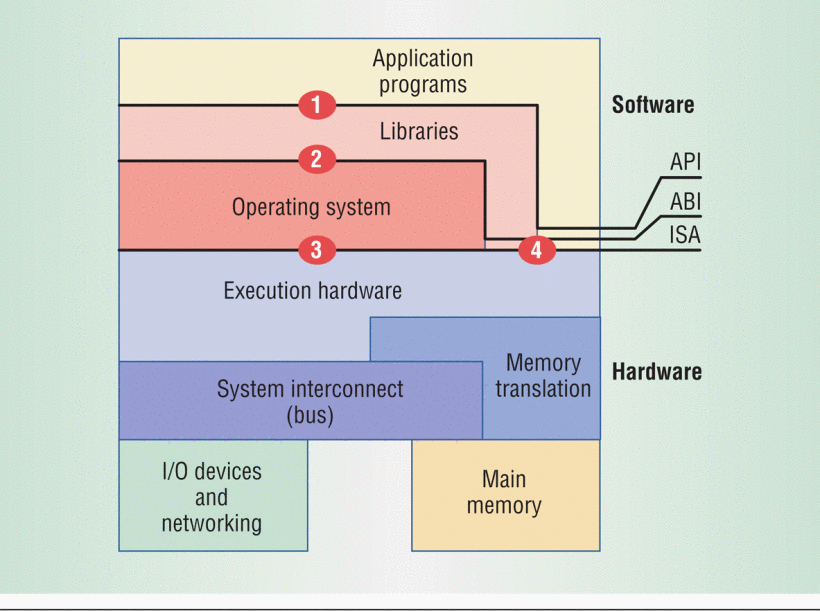
\includegraphics[scale=0.3]{assets/png/ca.png}
  \caption[Architektura počítačového systému]{Architektura počítačového systému \cite{book:iee:vm_architecture}}
  \label{figure:computer_architecture}
\end{figure}
\subsubsection{Instruction set architecture}
\label{chapter:virtualization:virtual_machine:computer_architecture:isa}
Instrukční sada neboli \textbf{ISA} definuje rozhraní mezi HW a SW. Tuto sadu je možné rozdělit na dvě části, a to na systémovou a
uživatelskou instrukční sadu. Rozhraní s~číslem 4 na obrázku \ref{figure:computer_architecture} reprezentuje uživatelskou
instrukční sadu, která obsahuje instrukce dostupné pro všechny uživatelské programy i knihovny. Rozhraní s~číslem 3 na stejném
obrázku pak reprezentuje systémovou instrukční sadu a zahrnuje instrukce dostupné pouze operačnímu systému. Tyto instrukce je
možné vykonávat pouze v~privilegovaném režimu procesoru a jsou zodpovědné za správu HW prostředků.
\subsubsection{Application binary interface}
\label{chapter:virtualization:virtual_machine:computer_architecture:abi}
Fyzické prostředky a zařízení dostupné ve fyzickém systému spravuje operační systém, který k~nim poskytuje přístup ostatním
programům skrze svoje rozhraní. Toto rozhraní s číslem 2 na obrázku \ref{figure:computer_architecture} se nazývá systémové
a společně s~uživatelskou částí \textbf{ISA} tvoří tzv. \textit{application binary interface} neboli \textbf{ABI}. Toto rozhraní
tedy neposkytuje aplikačním programům přímý přístup k~HW prostředkům, ale zprostředkovává je skrze systémová volání. Operační
systém tak může udržovat kompletní přehled o~využití jednotlivých prostředků.
\subsubsection{Application programming interface}
\label{chapter:virtualization:virtual_machine:computer_architecture:api}
Důležitou vrstvou softwarového vybavení počítače jsou uživatelské knihovny. Tyto knihovny skrývají implementační detaily
systémových volání a poskytují rozhraní pro vyšší programovací jazyky jako je C nebo C++. Společně s~uživatelskou
částí instrukční sady tvoří toto rozhraní nazývané \textit{application programming interface} neboli \textbf{API}.
Toto rozhraní je na obrázku \ref{figure:computer_architecture} označeno číslem  1. Uživatelské programy pak mohou využívat
tohoto rozhraní, což přináší výhody v~přenositelnosti na systémy, které nabízejí stejné \textbf{API}.
\section{Klasifikace virtuálních strojů}
\label{chapter:virtualization:clasification}
Aby bylo možné rozlišit jednotlivé typy virtuálních strojů, je nutné se podívat v~jaké části počítačové architektury operují
a tedy jakou vrstvu virtualizují. V~části \ref{chapter:virtualization:virtual_machine:computer_architecture} byly představeny 
tři dobře definovaná rozhraní počítačového systému a je logické, že virtualizační software bude virtualizovat nějaké z~nich.
Dle rozdělení \cite{book:iee:vm_architecture} mohou být virtuální stroje obecně rozděleny na následující dva druhy v~závislosti
na tom, které rozhraní počítačové architektury virtualizují:
\begin{itemize}
  \item \textit{systémové virtuální stroje},
  \item \textit{virtuální stroje v~procesech}.
\end{itemize}
Jak může být z~názvu patrné, \textit{systémové virtuální stroje} poskytují kompletní systémové prostředí, které podporuje
operační systém a jeho aplikace. Operační systém využívá ke svému běhu \textbf{ISA} fyzického systému. Systémový virtuální
stroj tedy musí poskytovat operačnímu systému stejné rozhraní jako OS očekává. Tímto způsobem nabízí operačnímu systému
přístup k~HW prostředkům fyzického stroje a~součástí tohoto způsobu zprostředkování může být i~virtualizace těchto prostředků.

Na druhou stranu procesy využívají mimo uživatelské části \textbf{ISA} také \textbf{ABI}. Vyšší programovací jazyky využívají
ještě abstraktnější rozhraní \textbf{API}. Virtuální stroje, které se specializují na virtualizaci těchto dvou systémových 
rozhraní, se nazývají \textit{virtuální stroje v~procesech}. Hlavním účelem tohoto typu virtuálního stroje je podpora jednoho
procesu. Její činnost začíná v~okamžiku vytvoření procesu a končí v~okamžiku jeho ukončení.

V~následujících kapitolách jsou popsané jednotlivé typy virtuálních strojů. Tato klasifikace \cite{book:iee:vm_architecture}
byla převzata a upravena podle požadavků práce.
\subsection{Terminologie}
\label{chapter:virtualization:clasification:terms}
Pro účely diplomové práce zde budou definovány některé pojmy, které se ve~virtualizované architektuře počítačového systému vyskytují. 

Přidání virtualizačního SW mezi dvě vrstvy počítačového systému vytvoří tři oddělené části. Tuto skutečnost popisuje
obrázek \ref{figure:system_vs_proces}, který zároveň ukazuje cílové umístění virtualizačního software v~případě systémových
virtuální strojů (b) a virtuálních strojů v~procesech (a). Softwarové vrstvy, které se v~hierarchii počítačového systému nachází
nad virtualizačním SW (je jim poskytováno rozhraní), se souhrnně nazývají \textit{guest}. V~případě systémových virtuálních strojů
se dá také mluvit o~\textit{guest OS}, což je operační systém běžící ve virtuální prostředí. Vrstvy nacházející se pod vritualizačním
SW se nazývají \textit{host}. Tyto vrstvy poskytují rozhraní virtualizačnímu SW, který ho zprostředkovává vyšším vrstvám hierarchie.

Poslední vrstvou systému je samotný virtualizační SW. V~případě systémových virtuálních strojů se standardně nazývá virtualizační
monitor neboli VMM. Pro virtualizační SW v~druhém typu virtuálních strojů se používá název \textit{runtime}. Tato vrstva tedy
virtualizuje prostředky nižších vrstev a prezentuje tak povahu systému jiným způsobem. 

Jak je naznačeno na obrázku \ref{figure:system_vs_proces}, typ virtuálního stroje je určen strukturou hosta a umístěním virtualizačního
SW. Systémové virtuální stroje se tedy skládají z~HW vrstvy a virtualizačního monitoru, který přímo operuje nad fyzickými prostředky
systému. V~případě virtuálních strojů v~procesech se vrstva hosta skládá z~HW a hostitelského operačního systému, ve kterém je spouštěn
\textit{runtime}.
\begin{figure}
  \centering
  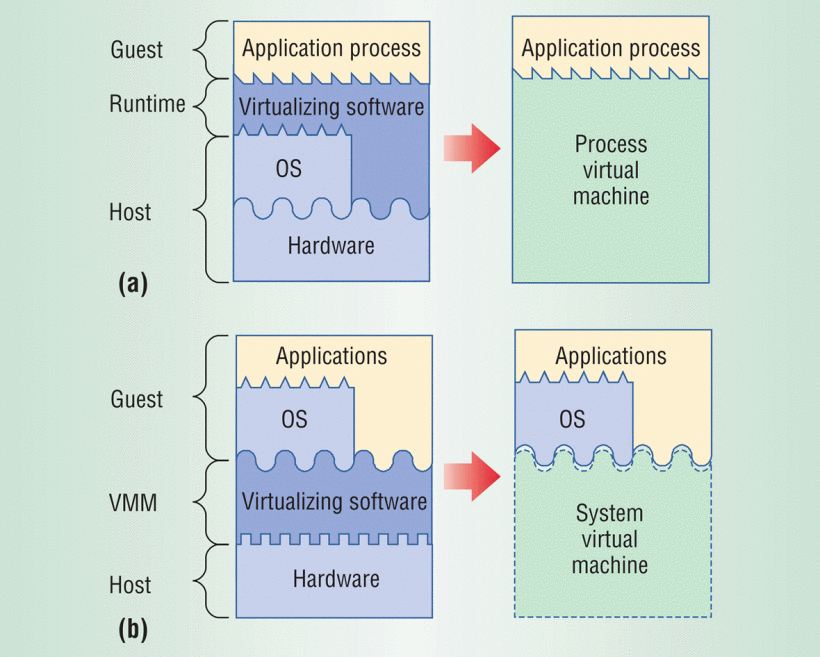
\includegraphics[scale=0.3]{assets/png/procesvm_vs_sysvm.png}
  \caption[Virtuální stroj v~procesu versus systémové virtuální stroje ]{Virtuální stroje v~procesech (a) versus systémové virtuální stroje (b) \cite{book:iee:vm_architecture}}
  \label{figure:system_vs_proces}
\end{figure}
\subsection{Virtuální stroje v~procesech}
\label{chapter:virtualization:clasification:process_vm}
Jak již bylo zmíněno, tento typ virtuálního stroje poskytuje uživatelským programům virtuální \textbf{ABI} nebo \textbf{API}.
Různé implementace těchto virtuálních strojů si kladou za cíl splnění různých kritérií. Některé se snaží zajistit přenositelnost
mezi různými počítačovými platformami a jiné se snaží optimalizovat instrukce uživatelského programu. Následovat bude stručný
výčet jednotlivých typů virtuálních strojů, které spadají do této kategorie virtualizace.      
\subsubsection{Virtualizace na úrovni OS}
\label{chapter:virtualization:clasification:process_vm:os_level_virtualization}
Jako virtuální stroj je možné považovat
operační systémy, které umožňují současný běh více procesů současně. Operační systém poskytuje každému procesu iluzi, že na
systému běží sám. Z~tohoto důvodu je nutné sdílet fyzickou paměť, CPU a jiná HW zařízení mezi běžícími procesy. Operační systém
poskytne každému procesu stejně velký izolovaný virtuální adresní prostor, který je mapován do fyzické paměti počítače. Procesor
je sdílen mezi procesy tak, že dochází k~tzv. přepínání kontextu, což znamená uložení všech registrů a načtení registrů
procesu, který má přidělený procesor. Přístup k~ostatním HW zařízením systému je řízen skrze systémové volání operačního systému.
Z~výše uvedených důvodů je možné říct, že OS poskytuje virtuální prostředí pro každý proces v~systému.

Dalším zástupcem virtualizace na úrovni OS je rozdělování zdrojů operačního systému nebo také vytváření zón. Pro tento účel
operační systém vytvoří pomocí procesů virtuální platformu, které je možné přidělit různé množství dostupných fyzických 
prostředků. Takto vytvořené virtuální stroje jsou většinou izolované na úrovni souborového systému, sítě a procesů. Jednotlivé
zóny se chovají jako nezávislé systémy a sdílejí jádro operačního systému s~hlavním operačním systémem. Jednotlivé úrovně 
izolace zajišťují, že jednotlivé zóny nemají žádné informace o~jiných zónách a ani je nemohou přímo ovlivnit.
\subsubsection{Emulátory a překladače}
\label{chapter:virtualization:clasification:process_vm:emulation}
Jak bylo zmíněno výše, některé implementace těchto virtuální strojů jsou zaměřeny na přenositelnost programů mezi jednotlivými
počítačovými architekturami. Tyto virtuální stroje zpracovávají instrukce jiné instrukční sady, než které vykonává systém hosta a poté
je dynamicky překládají do této instrukční sady. Konkrétní implementace by mohla například umožňovat vykonávat programy zkompilované
pro architekturu IA-32 na systému s~architekturou SPARC. Tyto virtuální stroje se nazývají překladače nebo emulátory, jelikož
emulují prostředí dostupné na jiných architekturách a mapují ho do architektury hosta.    
\subsubsection{Virtuální stroje v~HLL}
\label{chapter:virtualization:clasification:process_vm:hll_vm}
Virtuální stroje napsané ve vyšších programovacích jazycích přímo navazují na výše popsané téma přenositelnosti mezi platformami.
Nevýhoda emulátorů spočívá ve skutečnosti, že se specializují na překlad jedné instrukční sady do~druhé. Pokud by bylo nutné 
docílit přenositelnosti mezi všemi platformami, musel by být vytvořen emulátory pro každou kombinaci instrukčních sad. Jelikož
je toto řešení poněkud složité a náročné na implementaci, může být k~vytvoření virtuálního stroje použit právě vyšší programovací 
jazyk. Virtuální stroj napsaný v~konkrétním HLL se neopírá o~konkrétní architekturu, ale o~samotný programovací jazyk a jeho výhody.
Takto vytvořený virtuální stroj přijímá vlastní jazyk a využívá konkrétního HLL k~jeho provádění. Takto je zajištěna přenositelnost
programů, které jsou napsané v~jazyce virtuálního stroje, mezi systémy, na kterých jsou dostupné potřebné knihovny a samotná implementace virtuálního stroje.

Nejznámějším zástupcem této kategorie virtuálních strojů je Java virtual machine od společnosti Sun Microsystems. Tento virtuální
stroj provádí instrukce vyššího programovacího jazyka zvaného Java a dnes existuje mnoho implementací v~nejrůznějších programovacích
jazycích. Implementace HotSpot \cite{article:java:hotspot}, která je napsaná v~jazyce C++ a kterou v~dnešní době vyvíjí a 
udržuje společnost Oracle, je pravděpodobně neznámější a nejvíce využívanou implementací JVM.   
\subsection{Systémové virtuální stroje}
\label{chapter:virtualization:clasification:system_vm}
Druhým typem virtuálních strojů jsou tzv. \textit{systémové virtuální stroje}, které kompletně virtuálizují celou HW platformu.
Virtualizační software je většinou umístěn ihned nad HW vrstvu počítače a jeho hlavním úkolem je virtualizovat \textbf{ISA}. Tímto
způsobem \textit{systémové virtuální stroje} vytvářejí virtuální prostředí pro~běh operačního systému a jeho aplikací a dokonce
umožňují současný běh různých operačních systémů na jednom HW stroji.
\subsubsection{Virtuální počítače}
\label{chapter:virtualization:clasification:system_vm:virtual_computer}
Nejznámějším a pravděpodobně nejpoužívanějším zástupcem z~této kategorie virtuálních strojů jsou tzv. \textit{virtuální počítače}.
Tento typ virtuálního stroje umožňuje současný běh více operačních systémů na jednom fyzickém počítači. Všechny operační systémy
musí využívat instrukce stejné instrukční sady, kterou vykonává host. Tento typ virtuálního stroje žádným způsobem
nepřekládá instrukce do jiné instrukční sady.

Dle umístnění virtualizačního monitoru v~architektuře počítače, může být tento typ virtuálního stroje rozdělen do následujících kategorií:  
\begin{itemize}
  \item nativní VMM,
  \item hosted VMM.
\end{itemize}
Rozdíl mezi těmito dvěma typy spočívá v~umístění virtualizačního monitoru v~architektuře počítače. Zatímco 
\textit{nativní VMM} má přímou kontrolu nad HW počítače, \textit{hosted VMM} běží uvnitř operačního systému, který spravuje
HW prostředky. Oba tyto typy VMM jsou detailně popsány v~kapitole \ref{chapter:virtualization:vmm}.   
\subsubsection{Virtualizace celého systému}
\label{chapter:virtualization:clasification:system_vm:whole_system_virtualization}
V~případě, kdy virtualizovaný operační systém používá stejnou instrukční sadu jako fyzická platforma, má virtualizační monitor
za úkol spravovat přístup k~HW a sdílet ho mezi virtuální systémy. Pokud by bylo vyžadováno spouštění operačního systému
s~odlišnou instrukční sadou, musí být zajištěna emulace prostředí. Jinými slovy VMM musí vytvořit virtuální prostředí pro
konkrétní OS tak, aby si OS myslel, že je spuštěn na odpovídající HW platformě. Tento typ virtuálního stroje se nazývá
\textit{virtualizace celého systému}. Mimo instrukční sady mohou být virtualizovány i~některá I/O zařízení, která jsou
specifická pro konkrétní platformu.

Virtualizace celého systému se hojně využívá případech, kdy je nutné udržet v~chodu systémy, který běží na speciálních HW platformách.
V~tomto případě se vytvoří emulace celého prostředí a systém se přesune do takto vytvořeného prostředí. Systém i jeho aplikace
nepoznají žádný rozdíl, jelikož je celé prostředí virtualizováno. Tento typ virtuálního stroje je v~mnoha ohledech podobný
virtuálnímu stroji popsanému v~\ref{chapter:virtualization:clasification:process_vm:emulation}.
\subsubsection{Resource partitioning}
\label{chapter:virtualization:clasification:system_vm:partitioning}
Frekvence dnešních procesorů již není hlavním měřítkem jejich výkonnosti. Moderní procesory škálují svůj
výkon s~počtem výpočetních jader a díky tomu může být nezávisle spouštěno více výpočetních úloh najednou. Tato jádra jsou 
propojena sdílenou pamětí, která zajišťuje prostor pro ukládání dat a komunikaci. Tohoto faktu využívá technika zvaná 
\textit{resource partitioning}, která prostředky vícejádrového systému spojuje do nezávislých částí.

\textit{Hard partitioning} je technika, kdy jsou fyzické prostředky počítače rozděleny do disjunktních částí. Každá tato část
se chová jako nezávislý systém a~většinou má vlastní CPU (jádro), paměť, I/O zařízení i adaptér pro připojení k~síti. Jednotlivé
fyzické komponenty nebo jejich části jsou tedy přímo přiřazeny konkrétní části (partition) systému. V~takto rozděleném systému
pak může být současně provozováno několik instancí operačních systémů. Tato technika zajišťuje velkou míru izolace pro běžící operační
systémy, neboť každý OS má k~dispozici vlastní disjunktní prostředí, ve kterém může operovat. Pokud dojde k SW nebo HW chybě
v~jedné části (partition) systému, aplikace a OS běžící v~ostatních částech nejsou nijak omezeny.

Druhým přístupem k~rozdělování zdrojů je technika zvaná \textit{logical partitioning}. V~tomto případě fyzické prostředky nejsou
exkluzivně přiděleny jednotlivým operačním systémům, ale dochází k~jejich sdílení na SW úrovni. Ke sdílení procesoru a jeho jader
se například může používat časový multiplex, který umožňuje střídání OS ve využívání procesoru. Tato technika umožňuje lepší
využití fyzických prostředků než \textit{hard partitioning}, kde některé prostředky mohou kvůli malé zátěži zůstat nevyužity.
\section{Nasazení virtuální infrastruktury}
\label{chapter:virtualization:deployment}
Pro přechod k~virtuální infrastruktuře serverů existuje v~dnešní době několik důvodů. Jedním z~hlavních benefitů virtualizace
pro dnešní firmy a organizace je značná finanční úspora. Tato úspora se projevuje především ve snížení nákladů organizace na
pořizování a provoz fyzických zařízení. 

Mezi další benefity virtualizace patří především efektivní využití výpočetních zdrojů, vysoká dostupnost běžících aplikací nebo
vytvoření oddělených a~nezávislých prostředí pro vývoj, testování a nasazení software. Výhody zavedení virtuální infrastruktury
jsou podrobněji popsány v~následujících kapitolách, které se zabývají základními scénáři pro nasazení virtuální infrastruktury.
\subsection{Konsolidace}
\label{chapter:virtualization:deployment:consolidation}
Konsolidace serverů je proces sjednocování systémů z~více fyzických serverů na jeden fyzický server, který pro tyto systémy
poskytne virtuální prostředí pro jejich běh. Vstupem tohoto procesu je tedy několik systémů na fyzických serverech, na kterých
jsou spuštěny různé aplikace. Vstup procesu je zobrazen na obrázku \ref{figure:consolidation_img} vlevo. Výstupem konsolidace
je jeden fyzický server s~dostatečnými prostředky, na kterém jsou konsolidované systémy spuštěny jako virtuální počítače.
Výstup tohoto procesu je zobrazen na obrázku \ref{figure:consolidation_img} vpravo.
\begin{figure}
    \centering    
    \caption{Konsolidace serverů}
    \label{figure:consolidation_img}
\end{figure}
\subsubsection{Využití scénáře}
\label{chapter:virtualization:deployment:consolidation:use}
Dnes je zcela běžnou praxí provozovat jednu aplikaci na jednom dedikovaném serveru. Pokud aplikace využívá jen malé procento
výpočetních zdrojů daného serveru, může administrátor sjednotit více takovýchto serverů do jednoho. Pro~organizaci, která vlastní
tisíce takových serverů, může konsolidace výrazně zmenšit požadavky na prostor, spotřebu energie a provoz fyzických serverů.
Správnou konsolidací serverů může společnost docílit efektivního využití dostupných prostředků a tím výrazně snížit vynaložené
finanční prostředky \cite{oracle:virtualization:reasons}.

Rychlý vývoj technologií v~oblasti hardware je příčinou rychlého stárnutí některých systémů. Přechod ze staršího na nový může
být složitý, obzvláště v~případě, kdy systém potřebuje ke svému běhu speciální hardware. Aby bylo možné provozovat služby poskytované
těmito zastaralými systémy, můžeme je spustit jako virtuální počítač na modernějším hardware. Systém se bude chovat stejně jako
kdyby byl spuštěn na zastaralém hardware, zatímco výkonnost služby může těžit z~novější a výkonnější hardwarové vrstvy
\cite{oracle:virtualization:reasons}.
\subsection{Izolace}
\label{chapter:virtualization:deployment:isolation}
Dalším ze scénářů využití virtualizované infrastruktury je izolace aplikací. Proces izolace aplikací spočívá v~oddělení dvou
a více kritických aplikací spuštěných na jednom systému do nezávislých virtuálních prostředí. Vstupem je jeden systém
s~aplikacemi, které se mohou negativně ovlivňovat. Vstup izolačního scénáře je zobrazen na obrázku \ref{figure:isolation} vlevo.
Výstupem je několik nezávislých virtuálních počítačů, ve kterých jsou spuštěny jednotlivé aplikace. Výstup izolace aplikací
je zobrazen na obrázku \ref{figure:isolation} vpravo.
\begin{figure}
    \centering    
    \caption{Izolace aplikací}
    \label{figure:isolation}
\end{figure}
\subsubsection{Využití scénáře}
\label{chapter:virtualization:deployment:isolation:use}
V~dnešní době jsou útoky na aplikace vystavené do internetu běžnou záležitostí. Pokud útočník využije nějaké zranitelnosti 
aplikace, může v~některých případech získat kontrolu nad celým systémem. V~takovém případě jsou ohrožena všechna data a 
aplikace, které jsou na daném systému spuštěny. V~tomto případě je vhodné využít virtualizaci a rozdělit aplikace do nezávislých
prostředí.

Jedním z~příkladů ohrožení systému může být útok na výpočetní zdroje. Podstatou útoku je vyčerpání fyzických zdrojů systému,
což má za následek nedostupnost jeho služeb a v~některých případech i pád celého systému. Ve~   virtualizovaném prostředí lze
přidělit každému VM pouze určitou část prostředků a tím chránit celý systém před jejich vyčerpáním. V~případě napadení jednoho
VM sice dojde k~jeho vyřazení, ale ostatní VM a jejich služby mohou dále pokračovat v~provozu.
\subsection{Migrace}
\label{chapter:virtualization:deployment:migration}
Posledním diskutovaným scénářem nasazení virtualizované infrastruktury je migrace. Jedná se o~proces přesunutí systému z~jednoho
počítače na druhý. V~rámci virtualizace bude předmětem migrace systému na počítač s~běžícím VMM, který zprostředkovává
virtuální prostředí. Výstupem procesu je systém, který do něj zároveň vstupuje. Rozdíl je v~tom, že daný systém je na konci procesu
spuštěn ve virtuálním prostředí jiného VMM. Dle typu migrovaného systému je možné rozdělit scénář na dva typy.
\subsubsection{Migrace VM}
\label{chapter:virtualization:deployment:migration:virtual}
Migrací virtuálního stroje se rozumí přesun VM mezi dvěma různými fyzickými stroji s~VMM. Tento přesun byl dříve možný pouze
v~případě, kdy oba stroje měly stejný HW, operační systém a procesor \cite{oracle:virtualization:reasons}. Tato možnost administrátorovi
umožňuje přesouvat virtualizované systémy na výkonnější hosty a tím umožňuje dynamicky regulovat využití fyzických prostředků
v~závislosti na aktuální zátěži systému.

Další výhodou zavedení virtualizované architektury je zajištění vysoké dostupnosti služeb. Virtualizace umožňuje zajistit 
redundanci ve smyslu spuštění služby na více serverech najednou. Ve~virtualizované architektuře můžou nastat dva typy selhání.
Prvním typem je selhání virtuálního počítače. Pokud dojde k~selhání některého VM, jiný VM převezme obsluhu požadavků a
v~minimálním čase dojde k~obnovení služby. Druhým typem je selhání celého VMM nebo fyzického hosta. V~tomto případě je nutné
provozovat více redundantních hostů pro virtuální počítače, které v~případě HW chyby převezmou obsluhu služby.

Proces migrace VM je demonstrován na obrázku \ref{figure:migration:virtual}, kde je zobrazena konfigurace před migrací
a po provedení migrace VM.
\begin{figure}
    \centering    
    \caption{Migrace virtuálního stroje}
    \label{figure:migration:virtual}
\end{figure}
\subsubsection{Migrace fyzického stoje na VM}
\label{chapter:virtualization:deployment:migration:physical}
Migrace fyzického stroje na virtuální stroj je proces, kdy dochází k~přesunu a virtualizaci systému z~fyzického stroje.
Vstupem je systém, který je provozován na fyzickém stroji bez VMM. Tato skutečnost je zobrazena na~obrázku 
\ref{figure:migration:physical} vlevo. Výstupem tohoto procesu je opět virtuální stroj běžící ve~virtuálním prostředí VMM.

Virtualizací serverů dochází k~uvolňování fyzického HW a~stejně jako v~případě konsolidace, může společnost značně ušetřit
na nákladech nutných k~provozu a~správě fyzických serverů. Obecně lze říct, že tento scénář přináší podobné benefity jako
v~případě konsolidace popsané v~kapitole \ref{chapter:virtualization:deployment:consolidation}.
\begin{figure}
    \centering    
    \caption{Migrace fyzického na virtuální stroj}
    \label{figure:migration:physical}
\end{figure}
\section{Virtualizační monitor}
\label{chapter:virtualization:vmm}
Jak již bylo zmíněno, virtualizační monitor je softwarová vrstva starající se o~virtualizaci fyzických prostředků hosta.
Vytváří virtuální prostředí pro běh virtuálních počítačů. Virtualizační monitor tedy vytváří iluzi pro každý virtuální počítač, která
mu umožňuje transparentně přistupovat k fyzickým prostředkům počítače.
\subsection{Režimy ochrany CPU}
\label{chapter:virtualization:rings}
Moderní procesory mají čtyři režimy ochrany paměti, které se značí čísly od~0 do~3. Nejvyšší režim ochrany má číslo 0 a je
označován jako režim \textit{kernel}. Procesor běžící v~tomto režimu má přístup ke~všem instrukcím instrukční sady a může 
přistupovat k~jakékoli paměti. Číslo 3 naopak znamená režim nejnižší ochrany a může využívat jen část instrukční sady, která
se nazývá uživatelská \textbf{ISA}. Tomuto režimu se říká \textit{user}. Většina operačních systémů používá právě 
dva výše zmíněné režimy ochrany a zbylé dva jsou nevyužité.

Operační systémy v~nevirtualizované architektuře hrají roli řídícího programu, a proto běží v~režimu \textit{kernel}. Ve~virtualizované
architektuře tuto roli přebírá VMM, a proto je potřeba, aby běžel v~nejvíce privilegovaném režimu. Řešením může být posunutí
OS virtuálního stroje do méně privilegovaného režimu, například na úroveň 1, zatímco VMM poběží na úrovni 0. Druhým řešením
je vytvoření nového režimu ochrany s~číslem -1, který bude speciálně pro VMM. Současné procesory řeší ochranu právě tímto
způsobem a podporují plnou virtualizaci v~HW \cite{cvut:presentation:virt2}.

Výsledkem je tedy znemožnění přístupu programů s~nižší úrovní ochrany k~paměti alokované programem z~vyšší úrovně ochrany.
Paměť VMM je ve~virtualizované architektuře chráněna proti přístupu z~OS virtuálního počítače a stejně tak je chráněna paměť
OS virtuálního počítače před přístupem z~jeho procesů.
\subsection{Požadavky na VMM}
\label{chapter:virtualization:vmm:demands}
Z~úlohy virtualizačního monitoru při virtualizaci systémů plyne několik základních požadavků, které by měl VMM splňovat.
Specifikace \cite{cvut:presentation:virt2} těchto požadavků byla převzata.
\subsubsection{Transparentnost}
\label{chapter:virtualization:vmm:demands:transparency}
Operační systém běžící ve virtuálním prostředí virtualizačího monitoru by se neměl dozvědět o~existenci VMM ani jiných VM,
se kterými ve skutečnosti sdílí prostředky hosta.

VMM tedy zachytává systémové volání operačních systémů na HW zařízení nebo na čtení z~paměti a transparentně je vyřizuje.
Operační systém virtuálního počítače si tak myslí, že komunikuje přímo s~HW. V~této fázi VMM využívá některých technik virtualizace
CPU, paměti nebo I/O zařízení, aby mohl sdílet prostředky mezi virtuální stroje.
\subsubsection{Izolace}
\label{chapter:virtualization:vmm:demands:isolation}
Virtualizační monitor vytváří virtuální prostředí, které by mělo izolovat jednotlivé instance OS. Každý virtuální stroj má 
svůj kontext procesoru i svoji virtuální paměť mapovanou do jiných oblastí fyzické paměti. Jednotlivé VM tedy nemohou
vzájemně ovlivňovat svoji činnost a pád jedné VM by neměl ovlivnit činnost ostatních.
\subsubsection{Ochrana}
\label{chapter:virtualization:vmm:demands:access}
Virtualizační monitor by měl být chráněn proti přístupu z virtuálních počítačů. Operační systém virtuálního stroje 
je provozován v~privilegovaném režimu úrovně 1 (ring 1). Virtualizační monitor je provozován v~nejvíce privilegovaném režimu~\footnote[1]{Současné procesory podporují plnou virtualizaci v~HW. Mají speciální  režim ochrany úrovně -1 speciálně pro VMM \cite{cvut:presentation:virt2}}
úrovně 0. Pro operační systém virtuálního počítače to znamená, že nemůže přistupovat do paměti mapované pro VMM a privilegované
instrukce vyvolají systémové přerušení, které obsluhuje virtualizační monitor. V tomto okamžiku může docházet k emulaci chování
těchto privilegovaných instrukcí. 
\subsection{Typy VMM}
\label{chapter:virtualization:vmm:types}
V~následujících kapitolách jsou definovány tři základní druhy typické architektury virtualizačního monitoru, které se liší ve~způsobu
přístupu k~fyzickým prostředkům systému.
\subsubsection{Nativní VMM}
\label{chapter:virtualization:vmm:types:native}
Virtualizační monitor se nazývá \textit{nativní} nebo také \textit{bare-metal}, pokud má přímý přístup k~HW pomocí vlastních ovladačů.
Obvykle se \textit{nativní} VMM implementuje ve firmwaru počítače nebo jako hlavní řídící program, který se po~startu systému
zavede do~hlavní paměti a je mu předáno řízení. Tento přístup poskytuje nejvíce kontroly nad systémem a je také nejefektivnější,
protože VMM přístup k~HW zařizuje přímo.

Pokud virtualizační monitor nepodporuje určité typy procesorů nebo periferních zařízení některých HW platforem, může softwarové
vybavení VMM limitovat přenositelnost na tyto platformy \cite{cvut:presentation:virt1}.
\subsubsection{Hostovaný VMM}
\label{chapter:virtualization:vmm:types:hosted}
Druhým typem architektury je \textit{hostovaný} VMM. Tento název vychází z~faktu, že VMM využívá ke svému běhu existující operační
systém. Tento operační systém mu poskytuje rozhraní s~HW. Virtualizační monitor v~tomto případě neobsahuje ovladače k~HW,
protože jsou součástí operačního systému hosta. Aby mohl \textit{hostovaný} VMM správně pracovat, běží některé jeho části (jádro)
v~privilegovaném režimu procesoru společně s~operačním systémem hosta. Požadavky na HW zařízení jsou jádrem VMM přesměrovány
do komponenty VMM, která neběží v~privilegovaném režimu. Tato komponenta dále zavolá nativní rozhraní OS a požadavek je 
vyřízen operačním systémem hosta \cite{cvut:presentation:virt1}.

Tento typ virtualizace je v~dnešní době velice populární, protože umožňuje používat virtualizaci na systémech s~běžícím operačním 
systémem. Přenositelnost \textit{hostovaného} VMM je zcela určena přenositelností dané implementace. Na druhou stranu tento
typ VMM není vhodný pro nasazení do prostředí s~vysokými nároky výpočetní výkon, jelikož díky další vrstvě mezi HW a VMM není tak
efektivní jako \textit{nativní} VMM.
\subsubsection{Servisní VM}
\label{chapter:virtualization:vmm:types:servise}
Některé typy \textit{nativních} VMM vyžadují pro svoji plnou funkčnost jednu nebo více speciálních instancí VM. Tato instance
většinou slouží pro správu VMM a~ostatních instancí VM. Nicméně existují i virtualizační monitory, které využívají výhody
existujících OS a především jejich podpory velké škály HW ovladačů. V~tomto případě je OS spuštěn ve speciální instanci VM
a je společně s~jeho ovladači využíván jako komponenta VMM \cite{cvut:presentation:virt1}.